\documentclass[fontsize = 10pt, paper= a4,twocolumn,column_gap=5zw]{jlreq}

\usepackage[dvipdfmx]{graphicx}
\usepackage{color}
\usepackage{listings}
\usepackage{url}
\definecolor{OliveGreen}{rgb}{0.0,0.6,0.0}
\definecolor{Magenta}{cmyk}{0, 1, 0, 0}
\definecolor{colFunc}{rgb}{1,0.07,0.54}
\definecolor{CadetBlue}{cmyk}{0.62,0.57,0.23,0}
\definecolor{Brown}{cmyk}{0,0.81,1,0.60}
\definecolor{colID}{rgb}{0.63,0.44,0}
\lstset{
language={C},                   %言語の指定
basicstyle={\ttfamily\small},        %書体の指定
backgroundcolor={\color[gray]{.95}}, %背景色と透過度
keywordstyle={\color{blue}},         %キーワード(int, ifなど)の書体指定
commentstyle={\color{OliveGreen}},   %注釈の書体 
stringstyle=\color{Magenta},         %文字列
frame=single,                        %枠縁(leftline,topline,bottomline,lines,trBL,shadowbox, single)
numbers=left,                        %行番号表示
numberstyle={\ttfamily\small},       %行番号の書体指定
breaklines=true,                     %折り返し(自動改行)
breakindent = 10pt,                  %自動改行後のインデント量(デフォルトでは20[pt])	
tabsize=2,                           %タブの大きさ
captionpos=t                         %キャプションの場所(t,b : "tb"ならば上下両方に記載)
}
\renewcommand{\lstlistingname}{図} % キャプション名の指定

\begin{document}

\title{統計分析法 第5週レポート}
\author{202212022 田島瑞起}
\date{2023/11/14}
\maketitle
\section{設問1}
平均値の表
\begin{lstlisting}[basicstyle=\ttfamily\footnotesize, frame=single, caption=s2212022-1.c ,label=s2212022-1.c]
    A_jp A_math  A_eng   B_jp B_math  B_eng   C_jp C_math  C_eng 
    78.50  66.90  70.05  80.10  72.40  78.80  72.15  75.55  85.20 
    平均値に関しては,各要因ごとに見ても差があるように見える。
    \end{lstlisting}
標準偏差の表
\begin{lstlisting}[basicstyle=\ttfamily\footnotesize, frame=single, caption=s2212022-1.c ,label=s2212022-1.c]
    A_jp   A_math    A_eng     B_jp   B_math    B_eng     C_jp   C_math  C_eng 
    11.65513 13.36098 16.05738 10.17168 11.98859 11.38605 16.77177 16.76612 15.11918 
    \end{lstlisting}
    \begin{figure}
        \centering
        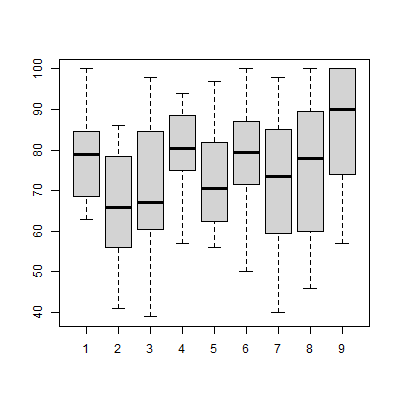
\includegraphics[width=4cm]{5-1.png}
    \end{figure}
\section{設問2}
\begin{lstlisting}[basicstyle=\ttfamily\footnotesize, frame=single, caption=s2212022-1.c ,label=s2212022-1.c]
    ANOVA分析を実行した結果下記結果がRのコマンドラインに表示された。
    Df Sum Sq Mean Sq F value Pr(>F)  
    class         2   1308   654.2   3.215 0.0426 *
    sub           2   1340   670.1   3.293 0.0395 *
    Residuals   175  35613   203.5                 
    ---
    \end{lstlisting}
\section{設問3}
優位水準0.05では"科目"の主効果が0.0396と導かれ,これは0.05を下回るものであるから,帰無仮説である「科目の平均値に差はない」は棄却される。

\section{設問4}
優位水準0.05では"クラス"の主効果が0.0426と導かれ,これは0.05を下回るものであるから,帰無仮説である「クラスの平均値に差はない」は棄却される。

\section{設問5}
(2)の結果により,class p = 0.0426 class F = 3.215, sub p = 0.0396 sub F = 3.293より,学群ごとに平均点の差が生じていることが示され,さらに科目ごとの平均点にも差が生じていることが示される。
この二つの結果を加味すると,各学群事に得意科目と不得意科目が存在する可能性が示唆される。
交互作用図を確認してみると,A群ではほかの学群に比べ数学が苦手科目である,B群はほかの学群に比べ国語が得意科目であり,C群はほかの学群に比べ英語と数学が得意科目であり,国語が苦手科目であることが読み取れる。
\begin{figure}
    \centering
    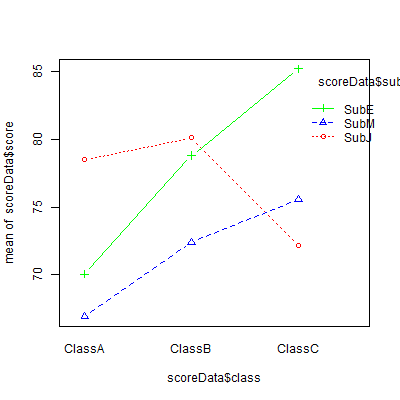
\includegraphics[width=4cm]{5-5.png}
\end{figure}

\section{ソースコード}
\begin{lstlisting}[basicstyle=\ttfamily\footnotesize, frame=single, caption=s2212022-1.c ,label=s2212022-1.c]
    #課題1
    Data <- Data <- read.table("score_ABC.txt",header=TRUE)
    MEAN.X <- c()
    NC <- ncol(Data)
    for(j in 1 : NC){
        MEAN.X <- c(MEAN.X,mean(Data[ ,j]))
    }
    SD.X <- c()
    for(j in 1 : NC){
        SD.X <- c(SD.X,sd(Data[ ,j]))
    }
    png("5-1.png", width = 400, height = 400)
    boxplot(Data$A_jp,Data$A_math,Data$A_eng,Data$B_jp,Data$B_math,Data$B_eng,Data$C_jp,Data$C_math,Data$C_eng)
    dev.off()
    
    #課題2
    
    classA <- factor(rep("ClassA", length = nrow(Data)))
    classB <- factor(rep("ClassB", length = nrow(Data)))
    classC <- factor(rep("ClassC", length = nrow(Data)))
    subJ <- factor(rep("SubJ", length = nrow(Data)))
    subM <- factor(rep("SubM", length = nrow(Data)))
    subE <- factor(rep("SubE", length = nrow(Data)))
    
    AJ <- data.frame(score = Data$A_jp, class = classA, sub = subJ, student = 1:nrow(Data))
    AM <- data.frame(score = Data$A_math, class = classA, sub = subM, student = 1:nrow(Data))
    AE <- data.frame(score = Data$A_eng, class = classA, sub = subE, student = 1:nrow(Data))
    
    BJ <- data.frame(score = Data$B_jp, class = classB, sub = subJ, student = 1:nrow(Data))
    BM <- data.frame(score = Data$B_math, class = classB, sub = subM, student = 1:nrow(Data))
    BE <- data.frame(score = Data$B_eng, class = classB, sub = subE, student = 1:nrow(Data))
    
    CJ <- data.frame(score = Data$C_jp, class = classC, sub = subJ, student = 1:nrow(Data))
    CM <- data.frame(score = Data$C_math, class = classC, sub = subM, student = 1:nrow(Data))
    CE <- data.frame(score = Data$C_eng, class = classC, sub = subE, student = 1:nrow(Data))
    
    scoreData <- rbind(AJ, AM, AE, BJ, BM, BE, CJ, CM, CE)
    
    # aovモデルの構築
    model <- aov(score ~ class + sub + class:sub, data = scoreData)
    
    # モデルの統計的な評価
    summary(model)
    
    #課題3
    #優位水準5%では"科目"の主効果が0.0396と導かれ,これは0.05を下回るものであるから,帰無仮説である「科目の平均値に差はない」は棄却される。
    
    #課題4
    #優位水準5%では"クラス"の主効果が0.0426と導かれ,これは0.05を下回るものであるから,帰無仮説である「クラスの平均値に差はない」は棄却される。
    
    #課題5
    #(2)の結果により,class p = 0.0426 class F = 3.215, sub p = 0.0396 sub F = 3.293より,学群ごとに平均点の差が生じていることが示され,さらに科目ごとの平均点にも差が生じていることが示される。
    #この二つの結果を加味すると,各学群事に得意科目と不得意科目が存在する可能性が示唆される。
    #交互作用図を確認してみると,A群ではほかの学群に比べ数学が苦手科目である,B群はほかの学群に比べ国語が得意科目であり,C群はほかの学群に比べ英語と数学が得意科目であり,国語が苦手科目であることが読み取れる。
    library(graphics)
    interaction.plot(
      x.factor = scoreData$class,
      trace.factor = scoreData$sub,
      response = scoreData$score,
      type = "b",
      legend = TRUE,
      col = c("red", "blue", "green"),  # 色は適宜変更
      pch = c(1, 2, 3)  # マーカーの種類は適宜変更
    )
    
    #課題6
    # A学群内の各科目ごとにTukeyの多重比較を実施
    tukey_result_math <- TukeyHSD(aov(Data$A_math ~ sub, data = scoreData))
    tukey_result_jp <- TukeyHSD(aov(Data$A_jp ~ sub, data = scoreData))
    tukey_result_eng <- TukeyHSD(aov(Data$A_eng ~ sub, data = scoreData))
    
    # 結果の表示
    print("Math Tukey Result:")
    print(tukey_result_math)
    
    print("Japanese Tukey Result:")
    print(tukey_result_jp)
    
    print("English Tukey Result:")
    print(tukey_result_eng)
    
    \end{lstlisting}

\end{document}